
\documentclass{beamer}
\usetheme{Wrexham}  
\usepackage{graphicx}

\usepackage{caption}
\usepackage{subcaption}
 
\begin{document}
\title{Compressive Sensing as a tool for Video Analysis}
\subtitle{}
\author{Rhian Davies \newline Idris Eckley, Lyudmila Mihaylova, Nicos Pavlidis}
\titlegraphic{ 
\includegraphics[height=.2\textheight]{logoEPSRC.png} \hspace{3cm} 
\includegraphics[height=.2\textheight]{logoSTORi.png}}
%\titlegraphic{
\includegraphics[height=.2\textheight]{logoEPSRC.png}}
\date{\today}

\begin{frame}[plain] 
  \titlepage
\end{frame}

  \begin{frame}{Motivation}
  \begin{figure}[h]
  \centering
  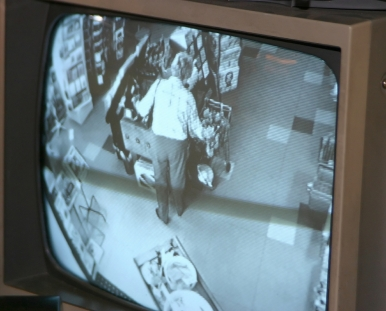
\includegraphics[height=5cm]{cctv}
 % \caption{Analysing CCTV footage}
  \label{fig:cctv}
\end{figure}  

\begin{quote}
\centering  ``Big Brother is Watching You.'' 
 \newline -  George Orwell, 1984  
\end{quote}  
 \end{frame}

%\begin{frame}
%  \frametitle{Nyquist – Shannon sampling theorem}
%If a function $X_t$ contains no frequencies higher than $N$ hertz, it is completely determined by giving its ordinates at a series of points spaced $\frac{1}{2N}$ seconds apart.
%GRAPH
%\end{frame} 

 \begin{frame}{What is compressive sensing?}
Compressive sensing is a method of \textbf{reducing the amount of data collected} from a signal without compromising the ability to later \textbf{reconstruct the signal accurately.}% This method will only work if the signal of interest is compressible. 

\begin{figure}[h]
        \centering
        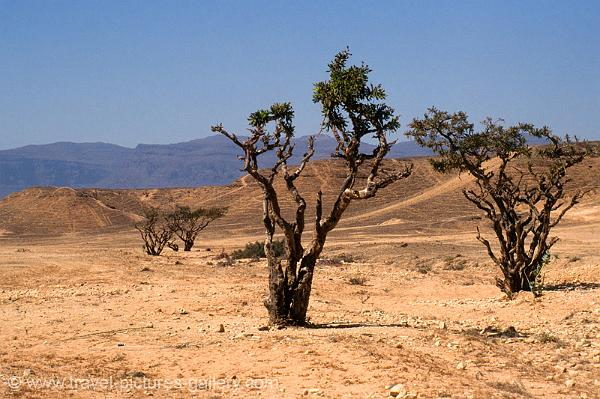
\includegraphics[width = 8cm]{sparseD.jpg}
       \end{figure}

\end{frame}

\begin{frame}{CS Methodology}
 % Assume that the signal of interest $\pmb{x}$ is of length N.
                 % \begin{itemize}
                 % \item Choose $M$, the number of measurements to take of $\pmb{x}$. $(M < < N).$
                   % \item Create a random measurement matrix $\pmb{\Phi}$ of size $M \times N$. This must satisfy the RIP. 
                   %   \item Calculate measurement $\pmb{y}$ according to equation \eqref{eq:1}.
                  %      \item Reconstruct $\pmb{x}$ using a recovery optimisation method.
                 % \end{itemize}

\begin{figure}[h]
        \centering
        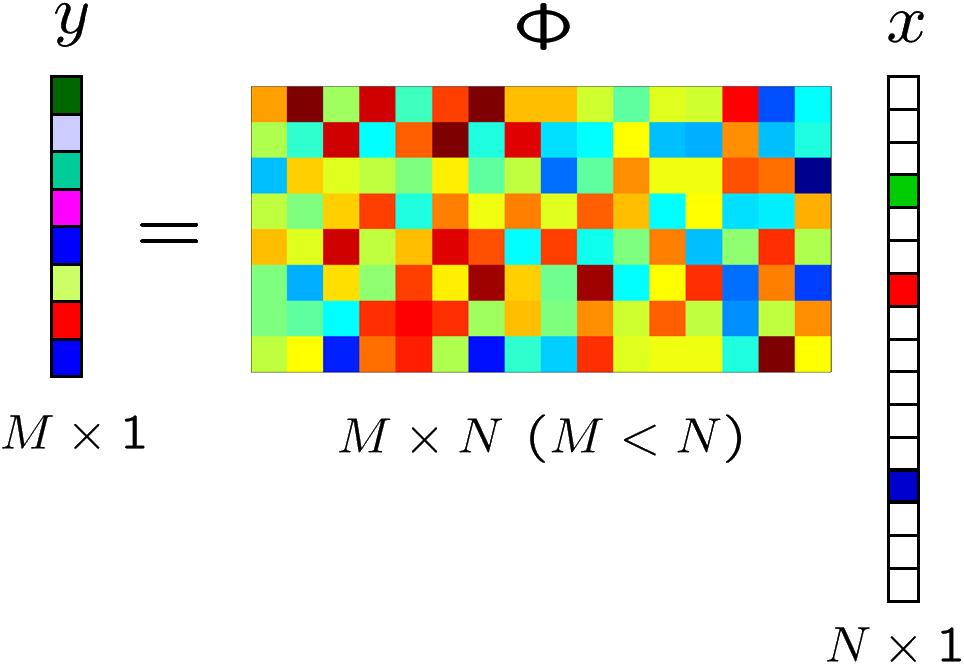
\includegraphics[width = 8cm]{csss}
        \caption{CS measurement process, courtesy of Volkan Cevher.}
      \end{figure}


%\begin{equation}
%  \label{eq:1}
%\pmb{y} =\pmb{\Phi x}
%\end{equation}
%Many vectors $\pmb{\hat{x}}$ can solve equation \eqref{eq:1}, but usually $\pmb{x}$ is the only sparse solution. Therefore if $\pmb{x}$ is known in advance to be sparse, it can in theory be reconstructed exactly from $M$ measurements.
\end{frame}

\begin{frame}{Restricted Isometry Property (RIP)}

  A matrix $\pmb{\Phi}$ satisfies the Restricted Isometry Property (RIP) of order $K$ if there exists a $\delta_K  \in (0,1)$ such that 
\begin{equation}
  \label{eq:4}
  (1 - \delta_k)||\pmb{x}||^2_2 \leq||\pmb{\Phi} \pmb{x}||^2_2 \leq (1 + \delta_k)||\pmb{x}||^2_2,
\end{equation}
for all $\pmb{x} \in \sum_K = {\pmb{x}:||\pmb{x}||_0 \leq K} $.
 
%If $\pmb{\Phi}$ satisfies the RIP with order $2K$, then $\pmb{\Phi}$ preserves the distance between any pair of $K$-sparse vectors, making the recovery procedure possible.
\end{frame}

      \begin{frame}{Recovery of sparse transforms}
        \begin{itemize}
\item $y = \Phi x$
          \item $\Delta(y, \Phi) = x$
\item Infinitely many solutions!
        \end{itemize}

\begin{equation*}
  \label{eq:3}
  \hat{x} = \text{arg} min_{y = \phi x} ||x||_0
\end{equation*}

\begin{equation*}
  \label{eq:3}
  \hat{x} = \text{arg} min_{y = \phi x} ||x||_1
\end{equation*}

Optimisation based on the $l_1$ norm can closely approximate compressible signals with high probability.

\end{frame}


\begin{frame}{Orthogonal Matching Pursuit}

 We shall define the columns of $\Phi$ to be $\varphi_1, \varphi_2, \hdots, \varphi_N$ each of length $M$. 

\begin{itemize}
%\item Inputs: Measurement matrix $\Phi$ and observations $y$.
%\item Initialize: $r_0 = y, \Lambda_0 = \emptyset$
%\item for $t=1, t:=t+1$ until stopping criterion is met \emph{do}
\item Step 1: Find the index for the column of $\Phi$ which satisfies $\lambda_t = \text{argmax }_{j=1,\hdots,N}|<r_{t-1}, \varphi_j>|$ 
\item Step 2: Keeps track of the columns used. $\Lambda_t = \Lambda_{t-1} \cup {\lambda_t}$, $\Phi_t = [\Phi_{t-1}, \psi_{\lambda_t}]$ 
\item Step 3: Update the estimate of the signal.  $x_t = \text{argmin}_x || v - \Phi_tx||_2$ .
\item Step 4: Update the measurement residual. $r_t =  y - \Phi_t x_t$.  
\item Output: Estimated sparse vector $\hat{x}$
\end{itemize}


  
\end{frame}
   
		% -- Frame 3-1
		\begin{frame}{Background Subtraction}
 \begin{figure}
                    \centering
                   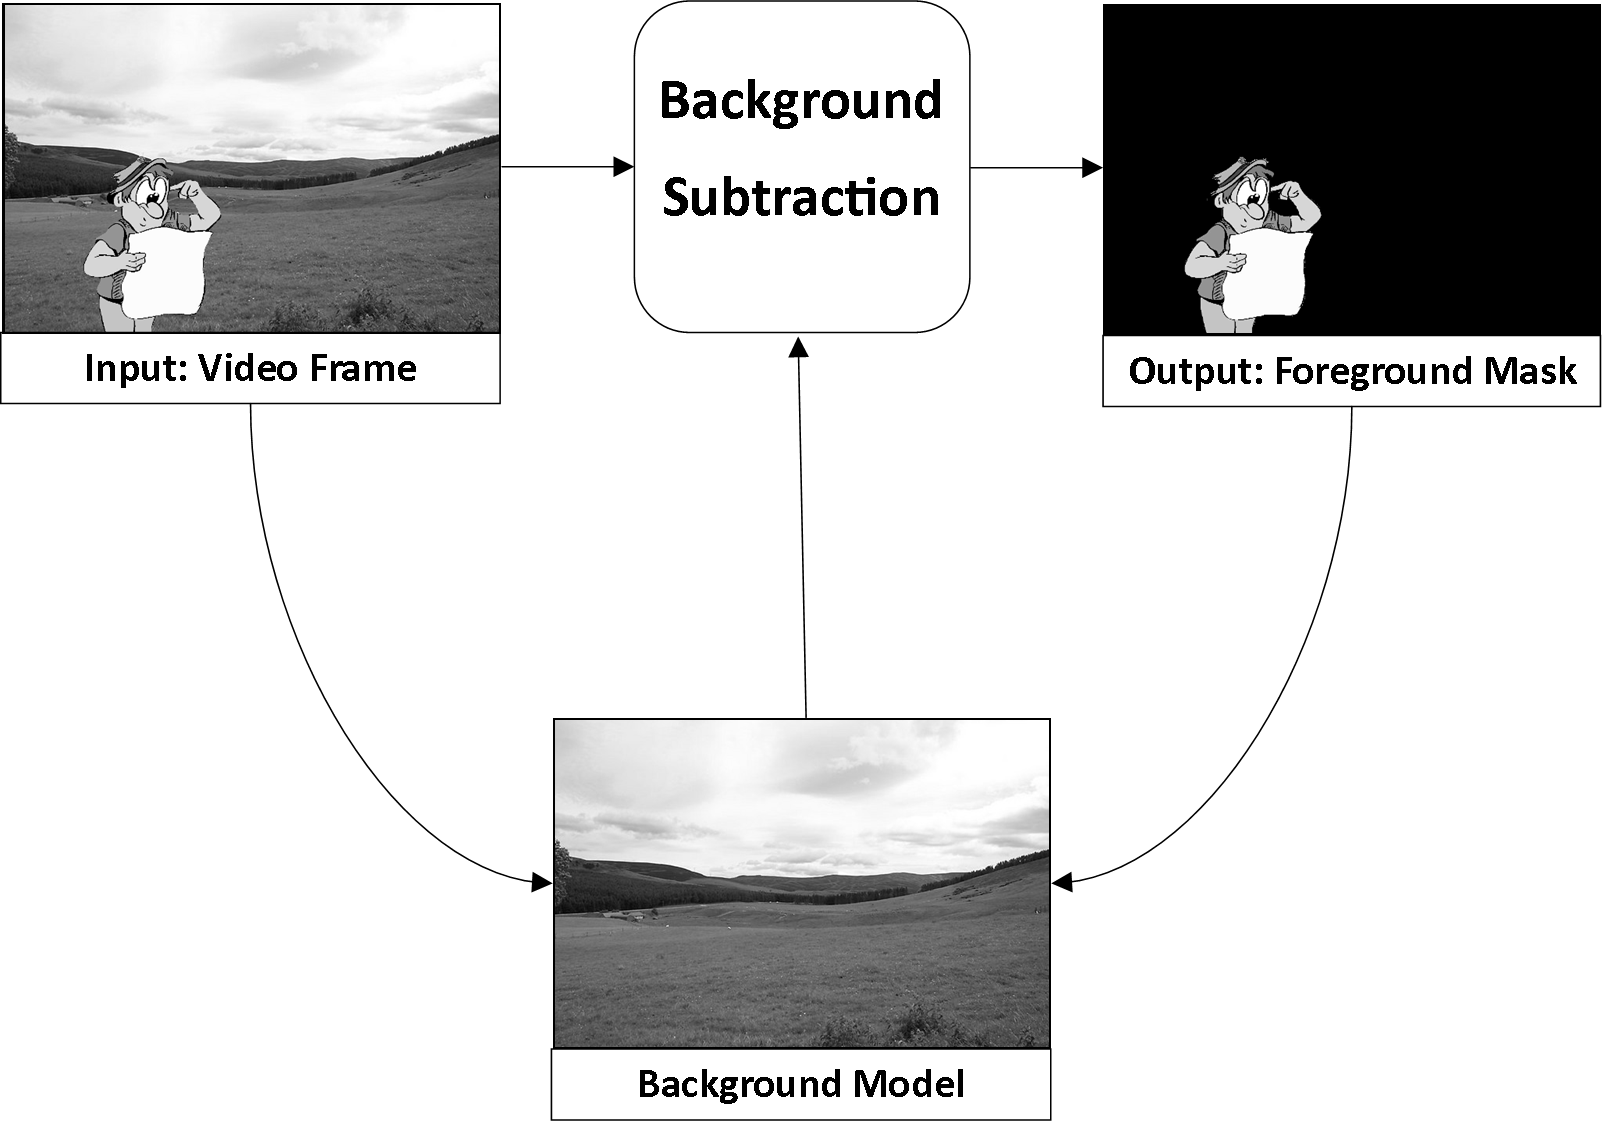
\includegraphics[width = 9cm]{backgroundsubtraction} 
\caption{The background subtraction process}
                  \end{figure}
 \end{frame}
                  \begin{frame}{Foreground sparsity}
                                      
                 
\begin{figure}[h]
  \centering
   \begin{subfigure}[b]{0.3\textwidth}
                \centering
                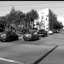
\includegraphics[width=\textwidth]{testFrameSp}
                \caption{Original frame}
        \end{subfigure}
\quad
\begin{subfigure}[b]{0.3\textwidth}
                \centering
                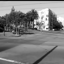
\includegraphics[width=\textwidth]{bgSp}
                \caption{Background Model}
                 \end{subfigure}
\quad
\begin{subfigure}[b]{0.3\textwidth}
                \centering
                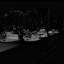
\includegraphics[width=\textwidth]{fgSp}
                \caption{Foreground Mask}
                 \end{subfigure}
\end{figure}

      \end{frame}

      
      % -- Frame 3-34 
      \begin{frame}{Background Subtraction with Compressive Sensing.}

\begin{enumerate}
\item Initialise a compressed background $y^b_0$.
\item Compressively Sense $y_t = \Phi x_t$.
\item Reconstruct   $\Delta (y_t - y^b_t)$
\item Update Background  $y^b_{t+1} = \alpha y_i + (1 - \alpha)y^b_i$
\end{enumerate}
\end{frame}

      \begin{frame}{Experimentation}
        \begin{figure}
          \centering
          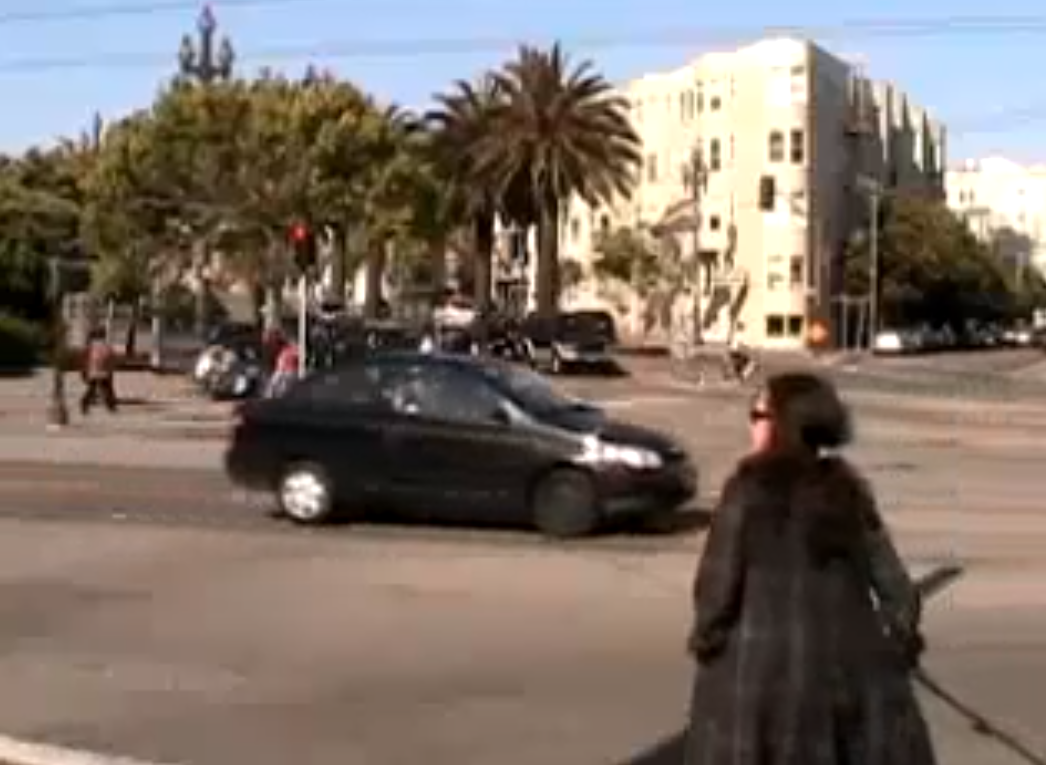
\includegraphics[width=7cm]{trafficvideo}
\caption{Sanfran test video courtesy of Seth Benton}
        \end{figure}
      \end{frame}
      
      % -- Frame 4-2
      \begin{frame}{Further Work}
        \begin{itemize}
        \item Choice of $\Phi$ and $\Delta$? 
\item More advanced methods of background subtraction.
\item Adapting with varying sparsity. 
\item Knowing when to reconstruct.
\item Exploiting the properties of natural images. 
        \end{itemize}
      \end{frame}





  \begin{frame}
    \frametitle{Any Questions?}
      \begin{figure}[h]
  \centering
  
\includegraphics[height=4cm]{questions.jpg}
 \end{figure} 
  \end{frame}

%  \begin{frame}
%    \frametitle{Impact}
%    
%  \end{frame}

 \end{document}
%%%%%%%%%%%%%%%%%%%%%%%%%%%%%%%%%%%%%%%%%%%%%%%%%%%%%%%%%%%%%%%%%%%%%%%%%%%%%%%%%%%%%%%%%%%%%%%%%%%%%%%%
%%%%%%%%%%%%%%%%%%%%%%%%%%%%%%%%%%%%%%%%%%%%%%%%%%%%%%%%%%%%%%%%%%%%%%%%%%%%%%%%%%%%%%%%%%%%%%%%%%%%%%%%%
\begin{frame}
  \frametitle{Analysing images mathmatically}

  \begin{itemize}
%  \item Assume images are black and white.
  \item An image is a matrix of pixels, with each pixel being represented by a number. 
\item This number is the grayscale intensity or luminance.
  \end{itemize}
  \begin{figure}[h]
\label{fig:grayscale}
    \centering
    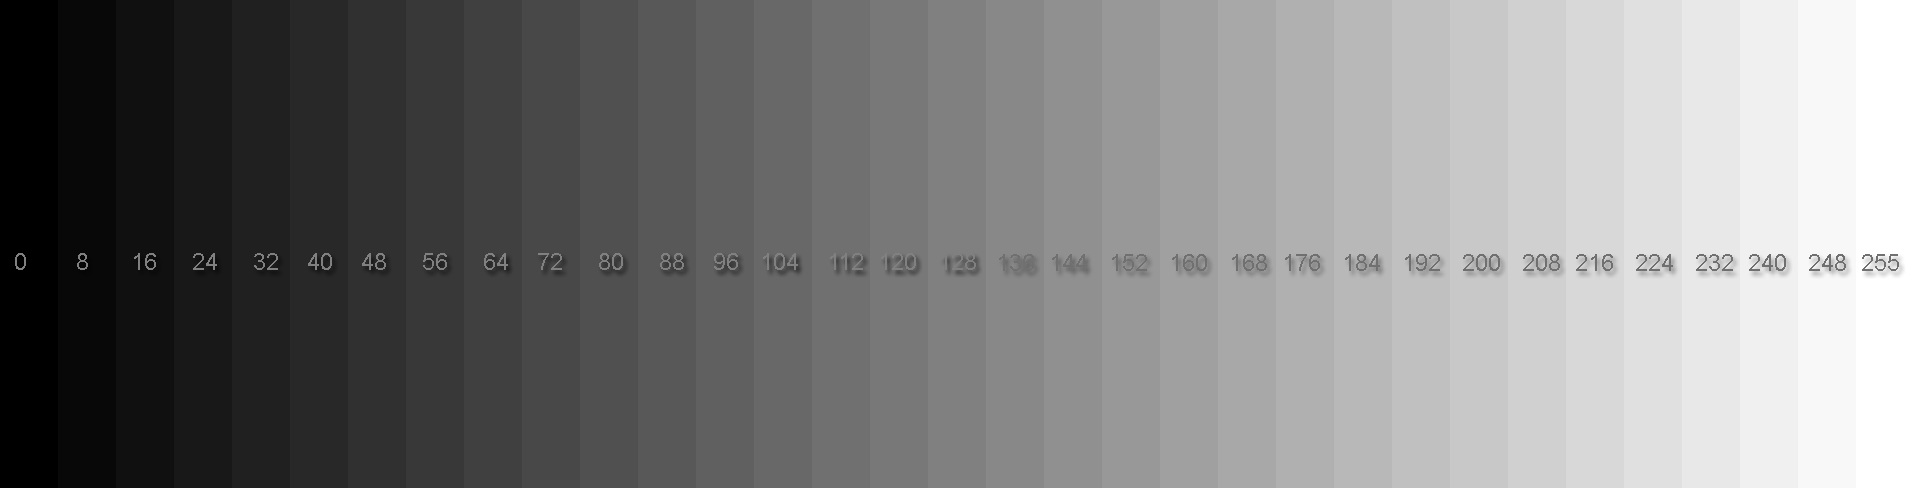
\includegraphics[height=2cm]{grayscale}
  %  \caption{Grayscale intensity}
    \end{figure}

\begin{figure}[h]
  \centering
  \[X_t =    \left( \begin{array}{ccc}
54 & 106 & 69 \\
220 & 7 & 3 \\
6 & 45 & 101 \end{array} \right)\] 
\end{figure}

 \begin{equation*}
    \label{eq:3}
X_t = [54,106,69,220,7,3,6,45,101]  \quad t= 1:T  
  \end{equation*}
\end{frame}

\begin{frame}
  \frametitle{Example}
Imagine you take a high quality picture and you wish to share this on the internet. If you used the full image uploading and viewing would take a long time. 

JPEG2000 compresses the image and but still retains the essential features of your image.

\begin{figure}
        \centering
        \begin{subfigure}[b]{0.4\textwidth}
                \centering
                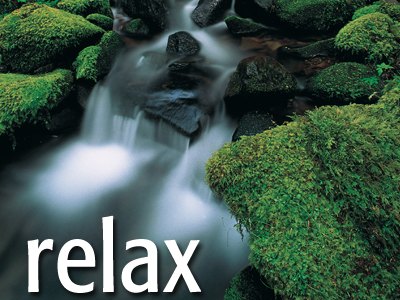
\includegraphics[width=\textwidth]{relax1}
                \caption{Original image}
                \label{fig:gull}
        \end{subfigure}
        \begin{subfigure}[b]{0.4\textwidth}
                \centering
                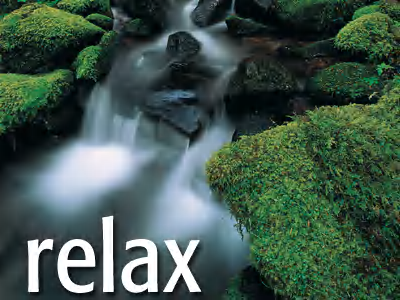
\includegraphics[width=\textwidth]{relax2}
                \caption{JPEG2000 compression}
                \label{fig:tiger}
        \end{subfigure}

\end{figure}

\end{frame}

      % -- Frame 3-2

%      \begin{frame}{Standard techniques for background subtraction}
%Frame differencing compares the  pixel intensity of the current frame and the previous frame and thresholds.Approximate median adapts a model of the background as each frame is read. Mixture of Gaussian models pixel intensity.These techniques have been studied in depth but don't work very well when dealing with occlusions, repetitive background motion and shadows, also termed ghosts.
%\end{frame}

      \vspace{10pt}
      
